\documentclass{article}
\usepackage[utf8]{inputenc}
\usepackage{indentfirst} % to have indent in the first paragraphs
\usepackage{geometry}
\geometry{
    a4paper,
    left=30mm,
    right=30mm,
    top=20mm,
    bottom=25mm,
}
\renewcommand{\baselinestretch}{1.5}
\usepackage{times}
\usepackage{latexsym}
\usepackage{float}
\usepackage{graphicx}
\usepackage{microtype}
\usepackage{hyperref}
\usepackage{amssymb}
\usepackage{amsmath}
\usepackage[makeroom]{cancel}
\usepackage{import}
\usepackage{xcolor}
% \usepackage{tikz}
\usepackage{filecontents}
\usepackage{adjustbox}

\usepackage[backend=biber, style=alphabetic, sorting=ynt]{biblatex}
\addbibresource{bibliography.bib}

\title{IN-STK5000 - Project 2 - Final}
\author{Aurora Poggi, Fábio Rodrigues Pereira, Nick Walker \\
\emph{Group 9}}
\date{December 2021}

\begin{document}

\maketitle

\tableofcontents

\clearpage

\section{Introduction}
\label{sec: Introduction}
In this project, we model the effect of vaccination against Covid-19 on a population. Our goal is to design a vaccination strategy which minimizes the rate of deaths in the vaccinated population. The first part of our report (\textbf{Section \ref{sec: Framework and Privacy issues}}) deals with describing the adaptive model training procedure, whereby we use a machine learning algorithm to iteratively learn a vaccination policy according to a specified utility function. We also discuss the issue of privacy in the data, and describe methods we have taken to ensure that the privacy of the treated population is safeguarded. In the second part of our report (\textbf{Section \ref{sec: Fairness}}), we analyze the issue of fairness in the results of our model as well as in the previous vaccination actions prior to our policy decisions. The final part of our report (\textbf{Section \ref{sec: Experiment Design}}) then deals with analysis of the historical data and further comparison to our improved policy, and further discussion of the comparative utility of each of them.

\subsection{Reproducibility}
\label{sec: Reproducibility}
This project can be reproducible by the code stored at our GitHub repository \href{https://github.com/fabiorodp/IN_STK5000_Adaptive_methods_for_data_based_decision_making/tree/main/project2}{https://github.com/fabiorodp/ IN\_STK5000\_Adaptive\_methods\_for\_data\_based\_decision\_making/tree/main/project2}. The results are achieved again with a high degree of reliability when the methodologies are replicated by the files
\textbf{\textit{main\_part\_a1.py}}, \textbf{\textit{main\_part\_a2.py}}, \textbf{\textit{main\_part\_b1.py}}, and \textbf{\textit{main\_part\_c.py}}.

\section{Framework and Privacy issues}
\label{sec: Framework and Privacy issues}

\subsection{Adaptive Model Procedure}
\label{sec: Adaptive Procedure}

To create our vaccination policy, our procedure begins by defining a "Trusted Curator" object in code. The Curator object provides a wrapper for the data which requires a user name and password to provide samples of the data. This is a layer of security for the data so that we can limit access to the population and vaccination information to researchers or other trusted parties who request access to the database. The data which is generated inside the Curator object (a population, from which we draw both features, actions, and outcomes, discussed later) is defined according to the simulator function provided in the Github repository\footnote{https://github.com/olethrosdc/ml-society-science/blob/master/src/covid/simulator.py}.

After creating our Trusted Curator, we then define our policy class object for vaccination. The first step is that we define that there are $3$ possible vaccines that can be given. These vaccines are simply numbered Vaccines $1$, $2$, and $3$ for reference. Our policy also includes a machine learning classifier (specifically, a Random Forest model) which will be adaptively learned and improved using the data as we observe the outcomes of the policy after each vaccination stage. The policy decides upon the expected utility, and a set of actions $A$ from a set of features $X$ provided by the Curator.

To measure our goal of minimizing the number of deaths (or equivalently, maximizing the rate of survival), we define an utility function $U$, such that
\begin{equation}
\label{eq: utility}
    U = \hat{p} = \frac{d}{T}
\end{equation}

\noindent where $d$ is the number of deaths and $T$ is the total number of people who contracted Covid-19 and were vaccinated.\footnote{For discussion of $\hat{p}$ as an unbiased estimator, see: \url{https://sites.warnercnr.colostate.edu/gwhite/wp-content/uploads/sites/73/2017/04/BinomialDistribution.pdf}} Broadly stated, this is to say that we wish to use a vaccination strategy which minimizes the number of deaths among the population of people who contract Covid-19 when all members of the population are vaccinated (and assuming that the vaccines are approved for all demographic groups by the competent authorities). 

After we obtain our data $X$ from the Curator, we then select our set of actions $A$ based on the expected utility 
\begin{equation}
\label{eq: expected utility}
    \mathbb{E}(U)=T \cdot \hat{p} = d
\end{equation}

\noindent of having vaccinated the population according to that set of actions. Thus, our set $A$ is selected as the set of individual actions $a$ which is estimated to produce the set of outcomes $Y$ with the minimum number of deaths, thereby minimising our utility function $U$.

When we select $X$, we draw a sample of $n = 10,000$ from the population for every vaccination stage. The first time the action selection is performed (1st vaccination stage), we randomly select a vaccine to give to each of the unvaccinated individuals in $X$, such that every unvaccinated individual receives one vaccine. We do not yet use the machine learning model of the policy to infer the outcome, since we have not yet fit it to an observed outcome. After this initially random selection of vaccines, we observe the outcome $Y$ of the vaccination. We are then able to calculate the sum of the deaths of individuals who were vaccinated and Covid-positive, under a random policy, for all possible vaccines combined, such that
\begin{equation}
\label{eq: expected utility 2}
    \begin{split}
        \mathbb{E}_\pi(U) &= T \cdot \hat{p}\\ 
        &= \cancel{T} \cdot \frac{d}{\cancel{T}}\\ 
        &= d\\
    \end{split}
\end{equation}

Still in the observe step, we save the triple $X, A, Y$ of features, chosen actions, and observed outcomes with which we will fit the model for our machine learning policy in the next vaccination stages. Next, a new vaccination stage can be initialized by drawing another $10.000$ individuals. These individuals are split into $2$ groups, vaccinated and not vaccinated. We call our utility method which will train the Random Forest model using the saved data from the previous vaccination step, plus the data of this current stage (recursively and adaptive part of the model). This model is fit on a bootstrapped and balanced set of training data which contains equal numbers of $y = death$ and $y = survive$ to ensure a model which does not over-fit to the $survive$ outcome. This model will subsequently be used to choose the specific vaccine which gives the highest probability of survival for each individual. Finally, the utility method computes the expected utility from the machine learning recommendations, which is the sum of the number of individuals that the model predicts death. This ML expected utility is compared with the mean of expected utilities observed from random vaccination policy. As the model is re-fit to the additional data in each stage, the objective of this process is to achieve an lower ML expected utility than expected utility for random vaccination choices. We observe that after several vaccination stages the model is able to predict actions for our policy which results in fewer deaths than the random policy, as shown in Figure \ref{fig: expected utility plot for each stage}.

\subsection{Machine Learning Policy}
\label{sec: Machine Learning Policy}

\begin{figure}[H]
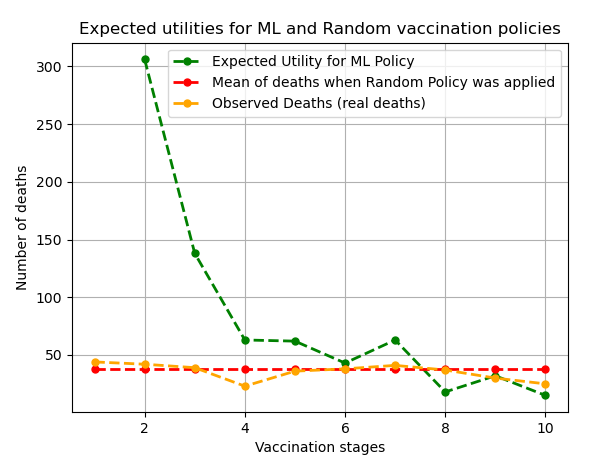
\includegraphics[width=10cm]{pictures/expected_utility_plot_for_each_stage.png}
    \centering
    \caption{A simulation of a 10 vaccination stages where decisions were selected from the following policy: Random, Random, Random, Random, Random, Random, Random, ML, ML, ML.}
    \label{fig: expected utility plot for each stage}
\end{figure}

In this section, we provide an overview of the training and decision process learned by our machine learning model. The result of our adaptive vaccination decision process is that the machine learning model must first learn sufficiently well to make predictions which are better than a random vaccination policy. When we test the policy update pipeline, we observe that for the first seven iterations, the model does not produce an action set which results in an expected utility better than the mean expected utility of the random policy (that is, the number of deaths predicted as a result of the model's estimation is higher than the expected deaths under the random policy). However, as the model is able to be trained on more data, the number of expected deaths from the learned actions drops to a level where we expect fewer deaths when the model suggested actions are taken. As shown in \textbf{Figure \ref{fig: expected utility plot for each stage}}, after $7$ vaccination stages the expected number of deaths from the ML Policy is lower than the average from the Random Policy (calculated over $7$ stages of Random Policy observations). We are then able to switch to using the learned model to determine our action rather than the random policy and vaccinate the population according to the model output. Through this process, we observe that the expected utility very closely matches the observed outcomes for the machine learning model, indicating that the model has fit the data appropriately and the estimated number of deaths from our ML policy is close to the true outcome (orange).

\subsection{Privacy}

In this section, we address the issue of privacy in the construction of our vaccination policy. As this database contains potentially sensitive information which may allow identification of the individuals described in it, we discuss several questions of privacy protection of the data and describe the methods by which we attempt to minimise the risk of data exposure.

\begin{itemize}
\item \textbf{\textit{Does the existence of this database raise any privacy concerns?}}

The database has several attributes that could be potentially important information that people would want to keep private. Most important among these is likely genetic data, which is highly sensitive and could potentially be used to find health conditions or susceptibility to health conditions. The age feature is also important as well, particularly because it is stored as a float, which suggests that this feature could be used to determine an exact date of birth. As dates of birth are frequently used for identity verification, this could pose a serious risk of identity theft to the individuals involved and therefore the resulting financial difficulties. Combined with gender this feature is also problematic, in consideration of the fact that as $87\%$ of Americans can be identified by birth date, gender and post code (see \textcolor{blue}{\cite{Dimitrakakis}}, p. 74), we can expect that similar conditions apply in all countries. Additionally, the vaccination status of individuals could also possibly be sensitive to certain individuals, as the revelation of this status could be the cause of interpersonal difficulties (e.g. bullying) among certain populations.  Furthermore, the income feature has potential to lead to similar outcomes if exposed. In particular, we may expect there is potential for making individuals with higher incomes more identifiable as targets for advertising or scams, and lower income individuals as targets for predatory lending or discrimination. Finally, comorbidities are an issue of significant privacy concern, as the release of an individuals medical conditions can similarly make them identifiable for targeted advertising as well as potential discrimination from employers, insurers, or others on the basis of these conditions.

\item \textbf{\textit{If the database was secret, but your analysis public, how would that affect privacy?}}

If the database was secret while the analysis was public, the privacy of the data would be more strongly protected. This scenario would prevent the direct use of the data by malicious actors for their own analysis of the population (perhaps attempting to de-anonymize the data by identifying the individuals from attributes). This setup of keeping the data secret would, however, compromise the ability of other researchers to reproduce the analysis that we present. One solution for this would be to create a synthetic data-set based on the distributions and attributes of the real data. This does rely on trust that the synthetic data is generated appropriately and conforms to the structure of the real data, but provides the opportunity for other researchers to apply the methods presented in the analysis. Moreover, it would be safer to only release real features which were most important in the original analysis, so that features which are not relevant to the task at hand cannot be used at all, reducing the exposition of the entire real data. Alternatively, it would also be possible to allow access to real data only through an API which implements a Differential Privacy Algorithm (e.g. \textit{$\epsilon$-differential privacy, $T$-fold adaptive composition, the Laplace mechanism, the exponential mechanism}, and other) under user registration and term of responsibility. It is essential to say that these differential privacy techniques are connected to learning theory and reproducibility (see \textcolor{blue}{\cite{Dimitrakakis}}, p. 79), therefore preferable than other simpler privacy approaches.

\item[(A)] \textbf{\textit{Explain how you would protect the data of the people in the training set.}}
%Laplace mechanism

The first way in which we protect the privacy of the people in the training set is to create our Trusted Curator object. As described in \textbf{Section \ref{sec: Adaptive Procedure}}, we create an object to manage access to the data, where username and password credentials are required to draw a sample from the data. This ensures that we can limit access to this database to trusted researchers or other individuals who contact the holders of the data to obtain access credentials. 

There are certain other transformations we can apply to the data in order to make it less individually identifiable. For instance, we can begin by looking at one of the more straightforward privacy-preserving applications, namely k-anonymity, because there are some \textit{quasi-identifiers} in our database that are particularly sensitive, e.g., age, gender, income. The first transformation we make is to transform the age variable from a float to an integer. This could be taken even further by transforming each to a range (buckets comprising for instance decades like 30-39, 40-49 and so on), however we do not implement this for our model. Similarly, this could be done for the income feature by bucketing income into different brackets rather than storing the exact number. This would impair calculating averages on these features, but it would strongly reduce how distinguishable the individuals in the data are. Another approach we can take is to use a \textit{Laplace Mechanism} which adds noise $\omega \sim Laplace$ to the sensitive attribute. This is the local privacy approach to \textit{Differential Privacy} on the Income feature, and so any functions applied to this feature (for instance calculating an average, or use in an estimator) will also be differentially private.

We therefore use three approaches within our Trusted Curator to protect the privacy of the people in the training set. The first, as mentioned previously is to transform the age feature from a float to an integer. This will then conceal the exact date of birth of the individual record. The second transformation we apply to the data is a \textit{Randomized Response} mechanism over the \textit{Gender} attribute. The mechanism draws a number from a $Bernoulli$ distribution (i.e. flips a fair coin) and if the number is greater than $0.5$, we again draw a number $n \in \{0, 1\}$ and insert this value in place of the original gender attribute (it may be the same as before). Therefore some number of the gender attributes will be flipped in the data. The third transformation to the data is to use the \textit{Laplace Mechanism} as described in the previous paragraph to add noise to the Income attribute. The advantage of applying a differential privacy method to this attribute is that any functions calculated from this attribute will also be differentially private.

\item[(B)] \textbf{\textit{Explain how would protect the data of the people that obtain treatment.}}

As an additional measure besides our Trusted Curator, we apply another differential privacy algorithm when calculating the utility of our vaccination policy. When we calculate the effect of our vaccination policy to assess the efficacy of our actions $A$, we observe the outcomes $Y$ from the vaccination group and use the number of deaths in this group (i.e. a sum) to evaluate our policy. This is a summary statistic over the population who received vaccinations, and so when calculating this from our data, we are able to make use of differential privacy algorithms in order to protect the privacy of the people who are given vaccination with outcomes $Y$. The use of such an algorithm when we calculate the statistic necessary to evaluate our policy will allow us to estimate the efficacy of our policy while hiding the data to a degree of privacy defined by $\epsilon$. As described previously with respect to the Laplace Mechanism, a differentially private result ensures that any functions calculated using this attribute will then be differentially private. 

The primary mechanism to protect the data of the people who are vaccinated in our policy is therefore an \textit{Exponential Mechanism} applied to the \textit{Death} column in our output $Y$. In the Exponential Mechanism, we have two variables which influence the modification of the data: the sensitivity of our utility function $\mathbb{L}(U)$ and $\epsilon$, which defines the degree of trade-off between accuracy of the calculation and preservation of privacy. The sensitivity of a function is defined as $\mathbb{L}(U)\stackrel{\Delta}{=}\underset{xNx}{\sup}|U(q,a,x) - U(q,a,x')|$, where two sets of data $x$ and $x'$ which differ only by one element. This means that here our sensitivity is merely $\mathbb{L}(U) = 1$, as the values in our data are binary, and thus a difference of one element in summing the deaths will be a difference of $1$. We are then free to choose the parameter $\epsilon$ and observe the effects on the utility of the ML policy.

\item[(C)] \textbf{\textit{Implement a private decision making mechanism for (b).}}

As described in (B) and following the instructions from the IN-STK5000\footnote{https://www.uio.no/studier/emner/matnat/ifi/IN-STK5000/h21/index.html} lab session on privacy\footnote{https://github.com/dhesse/IN-STK5000-Autumn21/blob/main/Session\%2007.ipynb}, we apply an \textit{Exponential Mechanism} to the \textit{Death} column in our output $Y$. In implementation this is to say that we calculate the probability of survival in the population, and repopulate the values of the column according to this probability distribution modified by our privacy guarantee $\epsilon$. This modification to the data therefore affects the calculation of the utility of our ML policy, and thus the actions we decide to take in the population. Our choice of $\epsilon$ is therefore of great importance not just due to the effect on how well the privacy of the data is preserved, but also because the effect of better preserving privacy may cause our policy to make a less accurate decision in our vaccination ML policy. As our choice of the privacy parameter $\epsilon \lim 0$, the algorithm returns a uniformly random result, and as $\epsilon \lim \infty$ the utility maximizing actions are chosen. Choosing the wrong value of $\epsilon$ would result in an ineffective policy which results in a higher number of deaths as a consequence. It is therefore crucial to understand the loss in utility of our policy for different values of $\epsilon$ in our privacy preserving decision making process, and so that we can choose a value of $\epsilon$ which minimizes deaths as outcomes of our policy while preserving privacy as much as possible.

\item[(D)] \textbf{\textit{Estimate the amount of loss in utility as you change the privacy guarantee.}}

When using the \textit{Exponential Mechanism} to preserve privacy in the vaccination outcomes, we define our parameter $\epsilon$. For this reason, we test our policy under differing values for $\epsilon$ and compare the resulting utility value of our policy between these values as well as without the privacy guarantee (our original results above). We wish to observe the difference in policy outcomes when different parameter values for $\epsilon$ are applied to the data.

\begin{center}
    \begin{table}[H]
    \centering
    \begin{adjustbox}{max width=\textwidth}
        \begin{tabular}{ |c| c c c c c c c c c | c | c |}
        \hline
          $\epsilon$ & \textbf{1} & \textbf{2} & \textbf{3} & \textbf{4}  & \textbf{5} & \textbf{6} & \textbf{7} & \textbf{8} & \textbf{9} & \textbf{Mean} & \textbf{loss} \\
         \hline
         0.5 & 172.0 &  161.0 &  125.0 &  108.0 &  80.0 &  99.0 &  79.0 &  86.0 &  84.0 &  110.4 & 48.4\\ 
         \hline
         0.6 & 157.0 &   79.0 &  132.0 &   87.0 &  82.0 &  83.0 &  45.0 &  59.0 &  46.0 &   85.5 & 23.5\\
         \hline
         \textcolor{blue}{0.7} & \textcolor{blue}{140.0} &  \textcolor{blue}{137.0} &   \textcolor{blue}{71.0} &   \textcolor{blue}{39.0} &  \textcolor{blue}{21.0} &  \textcolor{blue}{46.0} &  \textcolor{blue}{40.0} &  \textcolor{blue}{43.0} &  \textcolor{blue}{34.0} &   \textcolor{blue}{63.4} & \textcolor{blue}{1.4}\\
         \hline
         0.8 & 115.0 &  176.0 &  104.0 &   64.0 &  70.0 &  44.0 &  70.0 &  38.0 &  30.0 &   79.0 & 17.0\\
         \hline
         \textcolor{teal}{0.9} & \textcolor{teal}{134.0} &  \textcolor{teal}{113.0} &   \textcolor{teal}{94.0} &   \textcolor{teal}{61.0} &  \textcolor{teal}{29.0} &  \textcolor{teal}{39.0} &  \textcolor{teal}{28.0} &  \textcolor{teal}{33.0} &  \textcolor{teal}{25.0} &   \textcolor{teal}{62.0} & \textcolor{teal}{0.0}\\
         \hline
         \textcolor{violet}{real} & \textcolor{violet}{134.0} & \textcolor{violet}{113.0} & \textcolor{violet}{94.0} & \textcolor{violet}{61.0} & \textcolor{violet}{29.0} & \textcolor{violet}{39.0} & \textcolor{violet}{28.0} & \textcolor{violet}{33.0} & \textcolor{violet}{25.0} & \textcolor{violet}{62.0} & \textcolor{violet}{0.0}\\
         \hline
        \end{tabular}
    \end{adjustbox}
    \label{tab:utility-differences}
    \caption{Expected utility by vaccination stage for Non-private calculation (real) and values of $\epsilon$. The 'loss' column is the absolute value of the difference between the Mean of the non-private calculation and the $\epsilon$-differentially private calculation of that row.}
    \end{table}
\end{center}

\begin{figure}[H]
    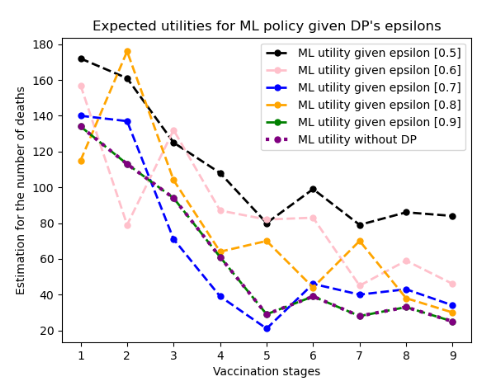
\includegraphics[width=10cm]{pictures/epsilons.png}
    \centering
    \caption{Expected utility of the ML policy under a given DP's epsilon.}
    \label{fig: epsilons}
\end{figure}

We tested several different values of $\epsilon$ between 0 and 1, in order to determine which presents the best tradeoff between privacy and performance. We first observe that for a choice of $\epsilon = 0.9$, we actually observe no impact on the utility of our actions. However, we also observe that we can reduce $\epsilon$ yet further while only minimally increasing the loss in utility, where $\epsilon = 0.7$ yielded a loss of utility of only 1.4. However at lower values than this the loss in utility quickly rises and we infer that the higher privacy guarantee begins to adversely affect the quality of the model more strongly.
\end{itemize}

\section{Fairness}
\label{sec: Fairness}
%What is fairness
In this document, we investigate the Covid-19 vaccination policy and decision making process we have designed previously in order to determine: 
\begin{itemize}
    \item Whether the policy, outcomes, and input data are fair, and 
    \item If unfairness exists, how it can be remedied. 
\end{itemize}

In order to do this we first need to define what we mean by fairness. Speaking in general terms, we can call a decision or outcome "fair" if the decision or outcome is not dependent on a $z \triangleq \text{\textit{sensitive attribute}}$ of a person, such that:
\begin{equation}
\label{eq: 1}
    \mathbb{P}_\theta^\pi(a|z) = \mathbb{P}_\theta^\pi(a)
\end{equation}

By sensitive attributes we mean characteristics of an individual which may place them into a group which is given different and often disfavorable treatment in comparison to other groups with differing characteristics. For instance, one example is the ongoing problem of gender discrimination against women which results in unfavorable outcomes in various domains such as pay, wherein the sensitive characteristic is the gender of the person. In an unfair scenario, a person with given qualifications $Q$ receives a different pay from someone with the same qualifications but differing in gender $G$. This can be described in somewhat informal notation as $Pay(Person\;|\;Q,G=Female) \neq Pay(Person\;|\;Q,G=Male)$. In short, we seek to avoid this unfair situation with respect to any sensitive variables which may be identified in the data. We can make use of two mathematical definitions of fairness in order to evaluate our system and determine whether the data or outcomes may be unfair to certain groups.

\subsection{Calibration}
\label{sec: Calibration}
The first formalized notion of fairness is \textit{Calibration}. The Calibration of a policy $\pi$ with parameters $\theta$ with respect to an outcome $y$, sensitive features $z$, and an action $a$ is defined (see \textcolor{blue}{\cite{Dimitrakakis}}) such that: 

\begin{equation}
\label{eq: Calibration}
    \mathbb{P}^\pi_\theta(y\;|\;a,z) = \mathbb{P}^\pi_\theta(y\;|\;a) \; \forall a, z
\end{equation}

This is to say that we want our outcomes to be independent of sensitive variables (the conditional probability of an outcome is the same regardless of the value of the sensitive variable, when the other attributes are the same). Concretely, we do not want our decision to result in unfair outcomes for example women as compared to men. It is important to note here that in our analysis, we mostly focus on fairness in \textit{outcome} rather than fairness in \textit{vaccination} in the sense of giving the same vaccines to different groups. This is because there may be valid reasons to give one vaccine to older groups and another to younger groups, as the efficacy of each vaccine may differ between these, and we are attempting to maximize the effectiveness of our policy in preventing deaths among the population. It is in this sense more important to focus on fairness in \textit{outcomes} to ensure that our policy is not neglecting the welfare of some groups in making decisions.

\subsection{Balance}
\label{sec: Balance}
The second notion of fairness is \textit{Balance}, which we can formalize as:

\begin{center}
$\mathbb{P}^\pi_\theta(a\;|\;y,z) = \mathbb{P}^\pi_\theta(a\;|\;y) \; \forall y, z$
\end{center}

Here we are instead looking at whether the action is taken independently of the sensitive attribute, given a true outcome $y$. This is to say that the probability of the action taken given the true outcome should be independent of the sensitive variable. As discussed above, in a medical context it may in some instances be valid to give different vaccines to different groups (particularly by $Gender$ and $Age$) as one vaccine may be more effective for one group than another.

\subsection{Fairness in Data \& Data Collection: Identifying Sensitive Variables}
\graphicspath{{pictures}}
To start our analysis, we look at the data to identify which variables might have implications on the fairness of vaccination policy and outcomes. The sensitive variables that stand out in the data are $Age$, $Gender$, and $Income$. These are attributes of a person which are both easily identifiable in practical terms (as opposed to finding out what genes a person has) and are often the subject of intentional and unintentional discrimination. For this reason it is then important to look at the data from the standpoint of fairness among the different groupings within these variables, ensuring that outcomes can be described as fair for both males and females, young and old, and across the income spectrum. 

We must first look at the distribution of the collected data $X$, as from the start we would like to know whether the data we are using to train our model fairly represents the population. The first and simplest attribute to analyze here is $Gender$, which is a binary attribute taking a value of $0$ or $1$. The general population of humans is more or less distributed $50-50$ between men and women, so we want to be sure that our data reflects this and that our model can be trained appropriately. If the data were for instance unbalanced such that women were underrepresented, any models trained on it would very likely make poorer decisions for women due to a comparative lack of data, leading to an unfair outcome.

\begin{figure}[H]
    \centering
    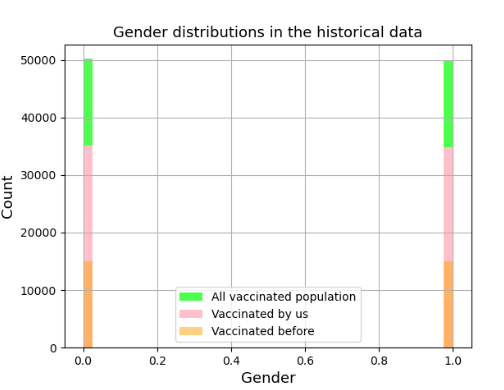
\includegraphics[width=10cm]{hd_gender_dist_version2.png}
    \caption{Gender distribution in the historical data after $10$ vaccination stages.}
    \label{hd_gender_dist}
\end{figure}

In \textbf{Figure \ref{hd_gender_dist}} we see that the distribution of men and women in our collected data is roughly half and half for each gender, which is in line with our expectation. From this standpoint we can say that the starting data is fairly collected with respect to $Gender$.

Next, we look at the age variable in the data. In contrast to $Gender$, the $Age$ variable is a floating point number in a range from $0$ to roughly $100$. For this reason we analyze the Ages of the population in "buckets", where we count the number of people in sub-ranges of ages, which is to say how many people are of an age between certain numbers ($0-30$, $30-60$, etc.). This distribution is not expected to be completely uniform, as a consequence of human mortality implying  that there will be fewer individuals above the age of $80$ than above $70$. Nonetheless, in order to find that the data is collected fairly, we should expect that each age group will be represented sufficiently to make informed decisions with their data. 

\textbf{Figure \ref{hd_age_dist}} shows the distribution of ages (not bucketed) in the initial data, showing a distribution with an average near $25$ and declining towards $100$ (with some examples well above $100$ which we might attribute to data entry error). This distribution reflects a relatively young population, but nonetheless is generally in line with what we might expect from a "population pyramid" with declining numbers of elderly individuals. Importantly we see sufficient numbers of data points for these individuals to be able to make reasonably informed decisions with a machine learning algorithm.

\begin{figure}[H]
    \centering
    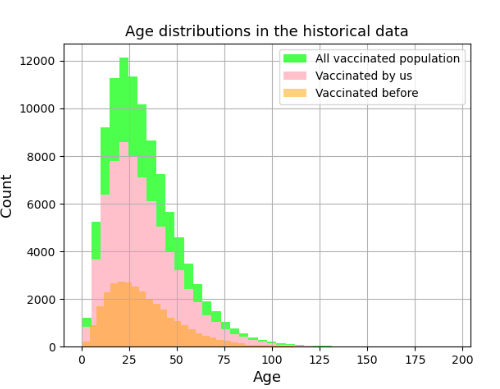
\includegraphics[width=10cm]{hd_age_dist_version2.png}
    \caption{Age distribution in the historical data after $10$ vaccination stages.}
    \label{hd_age_dist}
\end{figure}

Lastly, we analyze the $Income$ variable of the data to assess the distribution of incomes among the population. Here we expect that an unfairly collected set of data might be unreasonably skewed towards higher income, as oftentimes higher income individuals may have better access to healthcare and ability to take part in treatment programs. It is for this reason crucial that we appropriately collect data from low-income members of the population such that the vaccination decisions we take are not biased to give preferential outcomes according to income.

\begin{figure}[H]
    \centering
    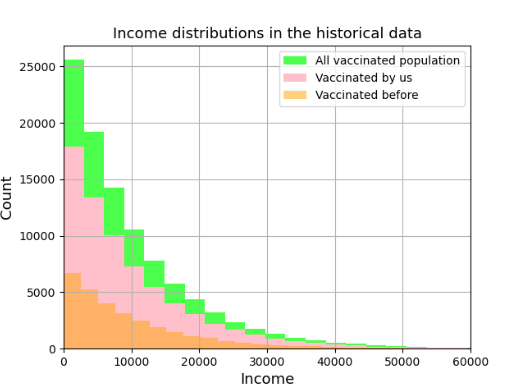
\includegraphics[width=10cm]{hd_income_dist_version2.png}
    \caption{Income distribution in the historical data after $10$ vaccination stages.}
    \label{hd_income_dist}
\end{figure}

\textbf{Figure \ref{hd_income_dist}} shows that the $Income$ variable in the data follows a power law distribution in which the largest chunk of individuals have no or little income, declining towards $0$ individuals as income increases. This kind of observation is discussed extensively in economics literature \textcolor{blue}{\cite{gabaix2016power}} and it is therefore unsurprising that comparatively few individuals make the highest incomes. For the same reason it appears appropriate to conclude that the data collection was not biased towards collection of higher income individuals' data, but also represents them to the degree that we would expect.

%We look at the amount of each group in the data and see if the incomes are in line with actual income distributions in the general population and if the data is representative of that with respect to income, age, gender.
%We also look at which groups get vaccinated and whether the rates of vaccination between them are different.

%We also analyze our decision making function and look at the outcomes and see how fair they are. We find that they are (fair|unfair) because our analysis shows this.

\subsection{Analyzing the Data \& Outcomes in Decision Making}

Following from our initial analysis of the data and its collection, we then look to investigate fairness as we make use of it for our decision making. As stated previously, we are attempting to design (or more specifically, train a machine learning model to produce) a vaccination policy which will result in the lowest number of deaths in the population. In the interest of fairness, we must look at the outcomes of this policy with respect to the sensitive variables identified in the previous section. An overview of this investigation can be demonstrated in the tables below. We look at the outcomes in three different cases: Among the previously vaccinated population (those with vaccines prior to our policy), among those vaccinated as a result of our policy, and the overall numbers among the whole vaccinated population

At a general level, we observe that our policy results in outcomes that are in line with the original trends of the data, which is to say that our policy does not disproportionately improve the outcome of one group relative to another when considering the sensitive variables. In the cases of the previously vaccinated population as well as the population we vaccinate, the probability of both receiving a specific vaccine (chance of action) and the probability of death (chance of outcome) are nearly equal across all groups of $Age$, $Gender$, and $Income$. One possible reason for the fair outcomes we observe from our policy is that our model is trained only using the top predictive features of death, which have in all cases been genes and comorbidities. Age is the most likely feature that we would expect to be predictive, but it has not been used in the models. While forgoing the use of sensitive variables in training a model is not in itself sufficient to guarantee fairness, in this case we suspect it may be enough to prevent unfair outcomes. It is also for this reason that, while it would be possible to design a utility function which balances fairness and raw utility e.g. a loss function $\mathcal{L}(U) = U + F(U)$ where we optimize via Stochastic Gradient Descent, in the case of our policy the observed outcomes suggest such an approach would be unnecessary.

%We can also describe the theory of SGD and fairness and why we don't need to use it since the outcomes seem to already be fair

\subsection{Calibration of Outcome When the Sensitive Variable Differs}

As mentioned in \textbf{Section \ref{sec: Calibration}} it is also instructive for us to look at the \textit{Calibration} of the policy with respect to the sensitive variables. First, we calculate the probability of an action given a sensitive variable (in accordance with the notions of fairness described in \textbf{Section \ref{sec: Introduction}}). We then measure the calibration of our decision making algorithm by analyzing the variation in the outcome with respect to the identified variables. This probability is calculated as described in \textbf{Section \ref{sec: Calibration}}.

Therefore, in this part of our analysis we calculate the conditional probabilities of both the outcomes and actions taken both in the original data and as a result of our policy. We wish to discover whether any discrepancies exist between groups in terms of either receiving certain vaccines or the risk of death in the data. 

%% for all vaccinated population
\begin{center}
\begin{table}[H]
\begin{adjustbox}{max width=\textwidth}
\begin{tabular}{ |c| c c c c c c c| }
\hline
A  & \multicolumn{7}{c|}{Z} \\
\hline
  & Age$\leq30$ &    $30<$Age$<60$ &     Age$\geq60$ &    Female &      Male &   $0k\leq$Income$<10k$ &    Income$\geq10k$ \\
\hline
 Vaccine1 &  0.326279 &  0.329881 &  0.329762 &  0.328845 &  0.327168 &  0.327888 &  0.328221 \\
 Vaccine2 &  0.361614 &  0.357654 &  0.363352 &  0.358166 &  0.362271 &  0.359787 &  0.360937 \\
 Vaccine3 &  0.312107 &  0.312465 &  0.306885 &  0.312989 &  0.310561 &  0.312325 &  0.310843 \\
 \hline
\end{tabular}
\end{adjustbox}
\caption{Table containing values of $\mathbb{P}(a|z)$ for '\textit{all vaccinated population}' space.}
\label{tab:1}
\end{table}
\end{center}

%% for vaccinated by us
\begin{center}
\begin{table}[H]
\begin{adjustbox}{max width=\textwidth}
\begin{tabular}{ |c| c c c c c c c|}
\hline
A  & \multicolumn{7}{c|}{Z} \\
\hline
  & Age$\leq30$ &    $30<$Age$<60$ &     Age$\geq60$ &    Female &      Male &   $0k\leq$Income$<10k$ &    Income$\geq10k$ \\
\hline
 Vaccine1 &  0.324264 &  0.327730 &  0.327526 &  0.328723 &  0.323096 &  0.325854 &  0.326046 \\
 Vaccine2 &  0.373828 &  0.368448 &  0.374041 &  0.368107 &  0.375377 &  0.370257 &  0.374250 \\
Vaccine3 &  0.301908 &  0.303822 &  0.298434 &  0.303170 &  0.301527 &  0.303889 &  0.299704
  \\ \hline
\end{tabular}
\end{adjustbox}
\caption{Table containing values of $\mathbb{P}(a|z)$ for '\textit{vaccinated by us}' space.}
\label{tab:2}
\end{table}
\end{center}

%% for vaccinated before
\begin{center}
\begin{table}[H]
\begin{adjustbox}{max width=\textwidth}
\begin{tabular}{ |c| c c c c c c c|}
\hline
A  & \multicolumn{7}{c|}{Z} \\
\hline
  & Age$\leq30$ &    $30<$Age$<60$ &     Age$\geq60$ &    Female &      Male &   $0k\leq$Income$<10k$ &    Income$\geq10k$ \\
\hline
Vaccine1 &  0.330939 &  0.334917 &  0.334935 &  0.329128 &  0.336595 &  0.332631 &  0.333243 \\
Vaccine2 &  0.333376 &  0.332372 &  0.338632 &  0.334971 &  0.331936 &  0.335371 &  0.330183 \\
Vaccine3 &  0.335685 &  0.332711 &  0.326433 &  0.335901 &  0.331470 &  0.331998 &  0.336574
  \\ \hline
\end{tabular}
\end{adjustbox}
\caption{Table containing values of $\mathbb{P}(a|z)$ for '\textit{vaccinated before}' space.}
\label{tab:3}
\end{table}
\end{center}

In \textbf{Tables \ref{tab:1}, \ref{tab:2}, \ref{tab:3}}, we observe the probability of actions taken dependent on the demographic groups. This is to say that each cell value describes the chance that a member of the column group will receive the vaccine in the row label. Overall, the vaccines are generally evenly distributed among the groups in the previously vaccinated population, as well as among the population our policy chooses to vaccinate. There is a slight preference for vaccination with $Vaccine2$ under our policy whereas in the original data no vaccine is more likely than the others for any group. However, for the purposes of fairness our policy succeeds in that this preference for choosing $Vaccine2$ applies to all demographic groups. If a difference between groups were observed here, it would not in itself indicate the policy is overall unfair, because as stated previously there may be a valid reason such as $Vaccine1$ or $Vaccine3$ working more effectively in preventing death in a particular group.

\begin{center}
    \begin{table}[H]
    \centering
        \begin{tabular}{ |c| c c c|}
            \hline
            & Vaccine1 &  Vaccine2 & Vaccine3  \\
            \hline
            All population &  0.328010 &  0.360210 &  0.311780 \\
            Vaccinated by us  &  0.325924 &  0.371723 &  0.302353 \\
            Vaccinated before &  0.332857 &  0.333455 &  0.333688
            \\ \hline
        \end{tabular}
    \caption{Table containing values of $\mathbb{P}(a)$ for all spaces (subsets).}
    \label{tab:Pa_summary}
    \end{table}    
\end{center}

\textbf{Table \ref{tab:Pa_summary}} summarizes the overall probability of receiving each vaccine among the population. Following the intuition behind equation (\ref{eq: 1}), \textbf{Table \ref{tab:Pa_summary}} should express the probability of outcomes given a fair policy, and subsequently we should observe \textbf{Tables \ref{tab:1}, \ref{tab:2}} and \textbf{\ref{tab:3}} displaying equivalent probabilities for each group (this is to say that no group has a disparate outcome when compared to the overall outcomes). We observe that this is the case, to some small degree of variation between groups.

Next we investigate the \textit{outcomes} of the vaccinations. This analysis relates to the $Calibration$ of the policy as mentioned before (\textbf{Section \ref{sec: Calibration}}), and we are calculating the probability of death given an action and a sensitive variable. Analysis of this data is then summarized by three sets of three tables, where the sets of tables describe outcomes of the overall vaccination, our vaccination, and previous vaccination, respectively. Each set contains a table describing the overall probability of death in that population, one describing the conditional probability of death given an action and demographic group, and a table showing the difference in outcome for a group compared to the overall outcome.

% calibration
% table for all population space
% $\mathbb{P}(y | a)$
\begin{center}
    \begin{table}[H]
    \centering
        \begin{tabular}{ |c| c c c|}
            \hline
            & Vaccine1 &  Vaccine2 & Vaccine3  \\
            \hline
            Dead &  0.004878 &   0.00422 &  0.004875 
            \\ \hline
        \end{tabular}
    \caption{Table containing $\mathbb{P}(y | a)$ for '\textit{all vaccinated population}' space.}
    \label{tab:simple_prob_py_a}
    \end{table}
\end{center}

%\textbf{Table \ref{tab:simple_prob_py_a}} describes the overall probability of death given an action ($Vaccine$) among the population. This simple metric gives us the indication that among the population as a whole, $Vaccine3$ is less effective in preventing death. The probability of death is approximately $0.001\%$ higher than $Vaccine1$, and $0.0005\%$  higher than $Vaccine2$. As $Vaccine1$ appears to be the most effective in preventing death, this is the vaccine that our policy learns to apply most frequently.

%Finally, \textbf{tables \ref{tab:6}, \ref{tab:8}, and \ref{tab:10}} show the probability of the outcome "death" given both the action and the sensitive variable. Here we are investigating the outcomes when broken down by demographic group. We compare these numbers with the overall probability of death in order to determine whether certain groups have outcomes worse than the overall probability.

% calibration
% table for all population space
% $\mathbb{P}(y | az)$
\begin{center}
\begin{table}[H]
\begin{adjustbox}{max width=\textwidth}
    \begin{tabular}{ |c| c c c c c c c|}
        \hline
          A  & \multicolumn{7}{c|}{Z} \\
          \hline
          & Age$\leq30$ &    $30<$Age$<60$ &     Age$\geq60$ &    Female &      Male &   $0k\leq$Income$<10k$ &    Income$\geq10k$  \\
        \hline
        Vaccine1 &  0.005281 &  0.004387 &  0.004738 &  0.005088 &  0.004665 &  0.004920 &  0.004806 \\
        Vaccine2 &  0.004712 &  0.004046 &  0.002150 &  0.003837 &  0.004601 &  0.004044 &  0.004521 \\
        Vaccine3 &  0.005087 &  0.004550 &  0.005091 &  0.004709 &  0.005044 &  0.004811 &  0.004987
         \\ \hline
    \end{tabular}
    \end{adjustbox}
    \caption{Table containing $\mathbb{P}(y | a, z)$ for '\textit{all vaccinated population}' space.}
    \label{tab:6}
\end{table}
\end{center}

\begin{center}
\begin{table}[H]
\begin{adjustbox}{max width=\textwidth}
    \begin{tabular}{ |c| c c c c c c c|}
        \hline
          A  & \multicolumn{7}{c|}{Z} \\
          \hline
          & Age$\leq30$ &    $30<$Age$<60$ &     Age$\geq60$ &    Female &      Male &   $0k\leq$Income$<10k$ &    Income$\geq10k$  \\
        \hline
        Vaccine1 &  0.000403 &  0.000491 &  0.000140 &  0.000210 &  0.000213 &  0.000042 &  0.000072 \\
        Vaccine2 &  0.000492 &  0.000174 &  \textbf{\textcolor{red}{0.002070}} &  0.000382 &  0.000381 &  0.000176 &  0.000301 \\
        Vaccine3 &  0.000212 &  0.000325 &  0.000216 &  0.000166 &  0.000168 &  0.000065 &  0.000112
         \\ \hline
    \end{tabular}
    \end{adjustbox}
    \caption{Table containing $| \mathbb{P}(y | a, z) - \mathbb{P}(y | a) |$ for '\textit{all vaccinated population}' space.}
    \label{tab:diff}
\end{table}
\end{center}

In \textbf{Tables \ref{tab:simple_prob_py_a} and \ref{tab:6}}, we apply the formula for calibration (\ref{eq: Calibration}) and obtain the conditional probabilities describing first the overall probability of death when given a vaccine, and secondly the probability of death given a vaccine and a sensitive attribute. Our goal here is to compare the demographic specific chances of death to the overall value, so that we can identify any groups which may have a disproportionately large risk of death relative to others. If there is no identifiable or substantial difference between the table values, then we can infer that the outcomes of the policy are fair. We can also observe that the chance of death observed with $Vaccine2$ is lower.

Comparing \textbf{Table \ref{tab:6} to Table \ref{tab:simple_prob_py_a}}, we can then summarize the results as in \textbf{Table \ref{tab:diff}}. Here we can observe the difference between each group's outcome and the overall outcome (probability of death). We can see that the highest disparity is among the most elderly ($60$ or older) who received $Vaccine2$. In this group, the chance of death was approximately $0.002\%$ higher than the  chance of death among all other groups. The next largest disparity is in outcomes for people $30$ years old or younger who have been given $Vaccine2$. The difference in chance of death for this group is larger than most other differences at $0.000492\%$, indicating that this group is also likely to be affected unfavorably by any decisions to give them $Vaccine2$. A near identical value is observed among people between the ages of $30$ and $60$ who received $Vaccine1$, indicating a similar conclusion. Subsequently, the next highest values are among the youngest age group when they received $Vaccine1$ and $Vaccine2$, indicating that $Vaccine2$ may provide a more unfair outcome when evaluating the results with respect to age. In any case, none of these values are especially large, so they do not indicate that the decisions of previous or current vaccination policy are grossly unfair to the age groups. All other deviations from the overall probability of death are negligible, and from this we have an indication that the policy is fair with respect to beneficial outcomes (survival).

% calibration
% table for vaccinated by us
% $\mathbb{P}(y | a)$
\begin{center}
\begin{table}[H]
\centering
    \begin{tabular}{ |c| c c c|}
    \hline
      & Vaccine1 &  Vaccine2 & Vaccine3  \\
    \hline
    Dead &  0.004827 &   0.00404 &  0.004589
     \\ \hline
    \end{tabular}
%\caption{Probability of death among recipients of each vaccine from our policy}
    \caption{Table containing $\mathbb{P}(y | a)$ for '\textit{vaccinated by us}' space.}
\end{table}
\end{center}

% calibration
% table for vaccinated by us
% $\mathbb{P}(y | az)$
\begin{center}
    \begin{table}[H]
    \begin{adjustbox}{max width=\textwidth}
        \begin{tabular}{ |c| c c c c c c c|}
            \hline
              A  & \multicolumn{7}{c|}{Z} \\
              \hline
              & Age$\leq30$ &    $30<$Age$<60$ &     Age$\geq60$ &    Female &      Male &   $0k\leq$Income$<10k$ &    Income$\geq10k$ \\
            \hline
            Vaccine1 &  0.005303 &  0.004200 &  0.004880 &  0.005454 &  0.004183 &  0.004924 &  0.004661 \\
            Vaccine2 &  0.004526 &  0.003736 &  0.002564 &  0.003865 &  0.004214 &  0.003967 &  0.004165 \\
            Vaccine3 &  0.004961 &  0.004173 &  0.004285 &  0.004599 &  0.004578 &  0.004462 &  0.004811
             \\ \hline
        \end{tabular}
        \end{adjustbox}
        \caption{Table containing $\mathbb{P}(y | a, z)$ for '\textit{vaccinated by us}' space.}
        \label{tab:8}
    \end{table}
\end{center}

\begin{center}
\begin{table}[H]
\begin{adjustbox}{max width=\textwidth}
    \begin{tabular}{ |c| c c c c c c c|}
        \hline
          A  & \multicolumn{7}{c|}{Z} \\
          \hline
          & Age$\leq30$ &    $30<$Age$<60$ &     Age$\geq60$ &    Female &      Male &   $0k\leq$Income$<10k$ &    Income$\geq10k$  \\
        \hline
        Vaccine1 &  0.000476 &  0.000627 &  0.000053 &  0.000626 &  0.000644 &  0.000096 &  0.000166 \\
        Vaccine2 &  0.000486 &  0.000304 &  \textbf{\textcolor{red}{0.001476}} &  0.000175 &  0.000173 &  0.000073 &  0.000125 \\
        Vaccine3 &  0.000372 &  0.000416 &  0.000304 &  0.000011 &  0.000011 &  0.000127 &  0.000222
         \\ \hline
    \end{tabular}
    \end{adjustbox}
    \caption{Table containing $| \mathbb{P}(y | a, z) - \mathbb{P}(y | a) |$ for '\textit{vaccinated by us}' space.}
    \label{tab:diff1}
\end{table}
\end{center}

We can continue this analysis on the level of the population whom we have vaccinate with our policy. Again we seek to uncover any disparities in the chance of death given a vaccine for each population, this time restricting ourselves to analyzing those individuals whose outcomes are a consequence of the actions we have taken. This is perhaps the most important group to look at in this way, because these are the results that are within our control as designers of the vaccination policy.

In \textbf{Table \ref{tab:diff1}} we summarize the difference in outcome per group versus the overall outcomes in the same manner as before. For this group, we observe the age group over $60$ years old given $Vaccine2$ had the largest difference in outcome from the overall probability, at approximately $0.0015\%$. Overall, the values are somewhat higher than among the overall population, but they are again very low and there are not substantial differences in outcomes for specific groups. One very interesting result that is also shown in this table is that the outcomes between males and females are identical in the case of $Vaccine3$  and nearly so in the case of $Vaccines$ $1$ and $2$. Additionally, when comparing to \textbf{Tables \ref{tab:pya vaccinated before} and \ref{tab:pyaz vaccinated before}} (further below), we observe that our policy has improved the outcomes for the lower income population at the cost of somewhat worsened outcomes for those with incomes above $10k$. At face value, this appears to swap outcomes between groups for no apparent advantage, however when we consider that as shown in \textbf{Figure \ref{hd_income_dist}}, by far the largest segment of the population is low income. In this regard, our policy represents an improvement in that the outcomes for a larger segment of the population are improved.

% calibration
% table for vaccinated before
% $\mathbb{P}(y | a)$
\begin{center}
    \begin{table}[H]
    \centering
        \begin{tabular}{ |c| c c c|}
            \hline
            & Vaccine1 &  Vaccine2 & Vaccine3  \\
            \hline
            Dead &  0.004993 &  0.004685 &  0.005479 \\
            \hline
        \end{tabular}
    \caption{Table containing $\mathbb{P}(y | a)$ for '\textit{vaccinated before}' space.}
    \label{tab:pya vaccinated before}
    \end{table}
\end{center}

% calibration
% table for vaccinated before
% $\mathbb{P}(y | az)$
\begin{center}
    \begin{table}[H]
    \begin{adjustbox}{max width=\textwidth}
        \begin{tabular}{ |c| c c c c c c c|}
            \hline
            A  & \multicolumn{7}{c|}{Z} \\
            \hline
            & Age$\leq30$ &    $30<$Age$<60$ &     Age$\geq60$ &    Female &      Male &   $0k\leq$Income$<10k$ &    Income$\geq10k$  \\
            \hline
            Vaccine1 &  0.005232 &  0.004814 &  0.004415 &  0.004236 &  0.005735 &  0.004911 &  0.005132 \\
            Vaccine2 &  0.005193 &  0.004851 &  0.001092 &  0.003766 &  0.005615 &  0.004243 &  0.005453 \\
            Vaccine3 &  0.005349 &  0.005356 &  0.006795 &  0.004942 &  0.006024 &  0.005556 &  0.005349 \\
            \hline
        \end{tabular}
        \end{adjustbox}
    \caption{Table containing $\mathbb{P}(y | a, z)$ for '\textit{vaccinated before}' space.}
    \label{tab:pyaz vaccinated before}
    \end{table}
\end{center}

\begin{center}
\begin{table}[H]
\begin{adjustbox}{max width=\textwidth}
    \begin{tabular}{ |c| c c c c c c c|}
        \hline
          A  & \multicolumn{7}{c|}{Z} \\
          \hline
          & Age$\leq30$ &    $30<$Age$<60$ &     Age$\geq60$ &    Female &      Male &   $0k\leq$Income$<10k$ &    Income$\geq10k$  \\
        \hline
        Vaccine1 &  0.000239 &  0.000179 &  0.000578 &  0.000757 &  0.000742 &  0.000082 &  0.000139 \\
        Vaccine2 &  0.000508 &  0.000166 &  \textbf{\textcolor{red}{0.003593}} &  0.000919 &  0.000930 &  0.000442 &  0.000768 \\
        Vaccine3 &  0.000130 &  0.000123 &  0.001316 &  0.000537 &  0.000545 &  0.000077 &  0.000130
         \\ \hline
    \end{tabular}
    \end{adjustbox}
    \caption{Table containing $| \mathbb{P}(y | a, z) - \mathbb{P}(y | a) |$ for '\textit{vaccinated before}' space.}
    \label{tab:diff2}
\end{table}
\end{center}

For the purpose of comparison and to investigate the fairness of vaccination decisions made prior to our policy, we perform the same analysis on the previously vaccinated individuals in the data. As mentioned previously, we can compare the outcomes among income groups and conclude that the previously vaccinated population displayed slightly better outcomes for those with income above $10k$. In this group, the largest difference in outcome was observed in the $60$ or older age group who received $Vaccine2$, at approximately a difference of $0.003\%$. The previous policy was also not especially unfair, as the differences in chance of death were not massively disparate. The same finding of similar outcomes among men and women also applies to the previously vaccinated population. This feature of the data may indicate that our policy was able to learn from the prior vaccinations in a way that preserved this aspect of fairness in vaccination with respect to gender. In the end, our decision policy achieved a better calibration score for $Age \geq 60$ ($0.001476$) in the worst case than the policy adopted for vaccination before ($0.003593$), showing that our decision distributes vaccines in a fairer way.

\subsection{Unifying view of fairness}
\label{sec: Unifying view of fairness}

Finally, we take a "unifying" view of fairness with which to investigate the policy, in that we want to measure any disparities in outcomes when measuring the calibration of the policy. This unifying measure of fairness with respect to the policy is defined (see \textcolor{blue}{\cite{Dimitrakakis}}) as follows:

\begin{equation}
\label{eq: F_calibration}
    \mathcal{F}_{\text{Calibration}}(\theta, \pi) \triangleq \max_{a, z} \sum_{i} \bigg{|}\mathbb{P}_{\theta}^{\pi}(y=i|a,z) - \mathbb{P}_{\theta}^{\pi}(y=i|a,z^{\prime})\bigg{|}
\end{equation}

This is, we evaluate the difference in outcomes between different values of sensitive attributes and select the largest absolute value of the difference. Our measure here gives an indication of how large the disparity in outcomes between different groups may be, where a larger difference indicates greater disparity. In the following tables, we summarize the $F$ values that we calculate over our policy for the sensitive variables we identified. This is as before broken down into the entire vaccinated population, the population vaccinated by our policy, and the previously vaccinated population, respectively.

\begin{table}[H]
    \begin{adjustbox}{max width=\textwidth}
        \begin{tabular}{|c| c c c c c c c|}
        \hline
          & Age$\leq30$ &    $30<$Age$<60$ &     Age$\geq60$ &    Female &      Male &   $0k\leq$Income$<10k$ &    Income$\geq10k$  \\
        \hline
         Age$\leq30$ &  0.000000 &  0.000895 &  \textbf{\textcolor{red}{0.002562}}  &  0.000874 &  0.000616 &  0.000668 &  0.000476 \\
        \hline
        $30<$Age$<60$ &  0.000895 &  0.000000 &  0.001896 &  0.000701 &  0.000555 &  0.000533 &  0.000475 \\
        \hline
        Age$\geq60$ &  \textbf{\textcolor{red}{0.002562}}  &  0.001896 &  0.000000 &  0.001688 &  0.002451 &  0.001894 &  0.002371 \\
        \hline
        Female &  0.000874 &  0.000701 &  0.001688 &  0.000000 &  0.000764 &  0.000207 &  0.000683 \\
        \hline
        Male &  0.000616 &  0.000555 &  0.002451 &  0.000764 &  0.000000 &  0.000557 &  0.000141 \\
        \hline
        $0k\leq$Income$<10k$ &  0.000668 &  0.000533 &  0.001894 &  0.000207 &  0.000557 &  0.000000 &  0.000477 \\
        \hline
        Income$\geq10k$ &  0.000476 &  0.000475 &  0.002371 &  0.000683 &  0.000141 &  0.000477 &  0.000000
        \\ \hline
        \end{tabular}
    \end{adjustbox}
\caption{Table containing the $\mathcal{F}_{\text{calibration}}$'s values for our sensitive variables $z$ for '\textit{all vaccinated population}' space.}
\label{tab:14}
\end{table}

\begin{center}
\begin{table}[H]
\begin{adjustbox}{max width=\textwidth}
    \begin{tabular}{ |c| c c c c c c c|}
    \hline
      & Age$\leq30$ &    $30<$Age$<60$ &     Age$\geq60$ &    Female &      Male &   $0k\leq$Income$<10k$ &    Income$\geq10k$  \\
    \hline
     Age$\leq30$ &  0.000000 &  0.001103 & \textbf{\textcolor{red}{0.001962}} &  0.000661 &  0.001120 &  0.000559 &  0.000642 \\
    \hline
    $30<$Age$<60$ &  0.001103 &  0.000000 &  0.001172 &  0.001253 &  0.000477 &  0.000723 &  0.000638 \\
    \hline
    Age$\geq60$ &  \textbf{\textcolor{red}{0.001962}} &  0.001172 &  0.000000 &  0.001301 &  0.001649 &  0.001403 &  0.001601 \\
    \hline
    Female &  0.000661 &  0.001253 &  0.001301 &  0.000000 &  0.001270 &  0.000530 &  0.000792 \\
    \hline
    Male &  0.001120 &  0.000477 &  0.001649 &  0.001270 &  0.000000 &  0.000740 &  0.000478 \\
    \hline
    $0k\leq$Income$<10k$ &  0.000559 &  0.000723 &  0.001403 &  0.000530 &  0.000740 &  0.000000 &  0.000349 \\
    \hline
    Income$\geq10k$ &  0.000642 &  0.000638 &  0.001601 &  0.000792 &  0.000478 &  0.000349 &  0.000000 
    \\ \hline
    \end{tabular}
    \end{adjustbox}
\caption{Table containing the $\mathcal{F}_{\text{calibration}}$'s values for our sensitive variables $z$ for '\textit{vaccinated by us}' space.}
\label{tab:15}
\end{table}
\end{center}

\begin{center}
\begin{table}[H]
\begin{adjustbox}{max width=\textwidth}
    \begin{tabular}{ |c| c c c c c c c|}
    \hline
      & Age$\leq30$ &    $30<$Age$<60$ &     Age$\geq60$ &    Female &      Male &   $0k\leq$Income$<10k$ &    Income$\geq10k$  \\
    \hline
     Age$\leq30$ &  0.000000 &  0.000418 &  0.004102 &  0.001427 &  0.000675 &  0.000951 &  0.000259 \\
    \hline
    $30<$Age$<60$ &  0.000418 &  0.000000 &  0.003759 &  0.001085 &  0.000921 &  0.000608 &  0.000602 \\
    \hline
    Age$\geq60$ &  0.004102 &  0.003759 &  0.000000 &  0.002674 &  \textbf{\textcolor{red}{0.004523}} &  0.003151 &  0.004361 \\
    \hline
    Female &  0.001427 &  0.001085 &  0.002674 &  0.000000 &  0.001848 &  0.000675 &  0.001686 \\
    \hline
    Male &  0.000675 &  0.000921 &  \textbf{\textcolor{red}{0.004523}} &  0.001848 &  0.000000 &  0.001372 &  0.000675 \\
    \hline
    $0k\leq$Income$<10k$ &  0.000951 &  0.000608 &  0.003151 &  0.000675 &  0.001372 &  0.000000 &  0.001210 \\
    \hline
    Income$\geq10k$ &  0.000259 &  0.000602 &  0.004361 &  0.001686 &  0.000675 &  0.001210 &  0.000000
    \\ \hline
    \end{tabular}
    \end{adjustbox}
\caption{Table containing the $\mathcal{F}_{\text{calibration}}$'s values for our sensitive variables $z$ for '\textit{vaccinated before}' space.}
\label{tab:16}
\end{table}
\end{center}

We first observe that among the population of all vaccinated individuals, the greatest disparity in outcome with respect to our measure in this section is between those who are $60$ years or older and those $30$ years old or younger, with a difference of roughly $0.0025\%$. What this says intuitively is that the difference in outcomes is greatest between these two groups when observing the entire vaccinated population. We can then compare this and other values in this table with \textbf{Table \ref{tab:15}}, which displays the same measure when calculated within the population of individuals vaccinated under our policy. In this case, the greatest difference is once between those aged $30$ years or less and those $60$ years or older, with a value of nearly $0.002\%$. The final table, \textbf{Table \ref{tab:16}}, displays the previous policy results, where the greatest difference lies between the oldest age group and males, standing with a difference of approximately $0.0045\%$. This is over twice the greatest difference in outcomes observed in the results of our policy, providing a good indication that our policy presents a substantial improvement in fairness when we evaluate outcomes by comparing group outcomes to one another. This is a more granular view of the issue and allows us to reason more specifically about why a policy could be considered fair, in that by fairness we somewhat inherently must be comparing between groups, rather than absolute values in outcomes. For this reason, despite the earlier analysis being somewhat inconclusive in determining whether previous policy or our policy is more fair (with the caveat that both are broadly fair in absolute terms), we can say in conclusion that our policy appears to make fairer decisions which result in less disparate outcomes for the population.

\section{Experiment Design \& Results}
\label{sec: Experiment Design}

To evaluate our policy and estimate how effective our decision making process is, we analyze and compare our policy results and those of the historical policy data.

\subsection{Estimations of Utility}

First, we estimate the utility of the historical policy as well as that of our policy. As before, this is calculated from the number of deaths in the population, that is to say that we calculate the probability of death. In order to provide error bars and a range on the estimate of this probability, we sample the results with replacement (bootstrapping) $1,000$ times, with a sample size of $25\%$ of the data. From this, we have a range of estimates on the true utility of both our policy results and the historical data.

\begin{figure}[H]
    \centering
    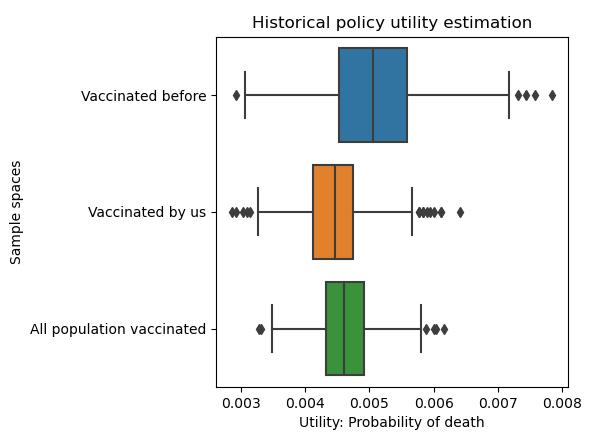
\includegraphics[width=10cm]{pictures/utility_estimations.png}
    \caption{Bootstrapped ($1000x$) estimations of utility for each space.}
    \label{fig: utility estimation}
\end{figure}

\textbf{Figure \ref{fig: utility estimation}} shows a box plot of the estimation of utilities of both policies and the overall when all vaccinated people are considered (this is to say the results of both policies combined). The previous policy (vaccinated before) has a much wider range of possible values, however the median value (and average) center around just over $0.005\%$ chance of death. Our policy by contrast has a lower median and mean probability of death, and the upper bounds of the estimate of our policy's utility are well within the bounds of the utility estimate on the previous policy. In \textbf{Table \ref{tab:describe}} we also report the key statistics for evaluating this, specifically that the mean estimate of probability of death for our policy was approximately $0.005\%$, lower than that of the previous policy. The \textbf{Table \ref{tab:measure_ut}} gives the measures of utility derived from the final results of the policy (that is, the calculation of the probability over the observed outcomes as a whole), where our policy achieved a lower probability of death in the population. From this we can see that our policy achieves the intended result of providing an improved approach to vaccination compared to the historical policy.

\begin{center}
    \begin{table}[H]
    \centering
    \begin{adjustbox}{max width=\textwidth}
        \begin{tabular}{ |c c c c|}
            \hline
            &  Vaccinated before &  Vaccinated by us &  All population  \\
            \hline
            mean & 0.005053 & \textcolor{blue}{\textbf{0.004458}} & 0.004618 \\
            \hline
            std & 0.000812 & 0.000505 & 0.000436 \\
            \hline
            min & 0.002925 & 0.002861 & 0.003280 \\
            \hline
            max & 0.007845 & 0.006408 & 0.006160
             \\ \hline
        \end{tabular}
        \end{adjustbox}
    \caption{Table containing some descriptive statistics for each (1000X) estimations of utility for each space.}
    \label{tab:describe}
    \end{table}
\end{center}

% %%% Measure of utilities - final values over the spaces
\begin{center}
    \begin{table}[H]
    \centering
    \begin{adjustbox}{max width=\textwidth}
        \begin{tabular}{ |c c c c|}
            \hline
            &  Vaccinated before &  Vaccinated by us &  All population  \\
            \hline
            Measure of utilities & 0.005052 & \textcolor{blue}{\textbf{0.004463}} & 0.00464
             \\ \hline
        \end{tabular}
        \end{adjustbox}
    \caption{Table containing the measure of utilities for each space.}
    \label{tab:measure_ut}
    \end{table}
\end{center}

\section{Conclusion}

In conclusion, our report has demonstrated a method of adaptively learning a Covid-19 vaccination policy. We have shown the overall method for constructing this, including the pipeline and model training, considerations of privacy issues and specific implemented methods to preserve privacy, and an evaluation of the fairness of our policy with comparison to the historical policy. We have then summarized our results with estimations of the utility of the different policies and a comparison which shows the improved effectiveness resulting from our policy after 10 stages of vaccination. In addition to the improved performance relative to the historical policy, we have shown in \textbf{Section \ref{sec: Fairness}} that our policy is additionally at least as and very likely more fair than the previous policy, and in \textbf{\ref{sec: Framework and Privacy issues}} described how our method is also able to respect the privacy of the population. In sum, the adaptive method presented in our report represents an improvement in determining vaccination policy by saving additional lives in this population and successfully addresses the key issues that arise in designing such a policy.

\addcontentsline{toc}{section}{References}
\printbibliography
\end{document}
